\documentclass[12pt,a4paper]{article}

\usepackage{style2017}
\usepackage{hyperref}

\hypersetup{
    colorlinks =false,
    linkcolor=blue,
   linkbordercolor = 1 0 0
}
\newcounter{numexo}
\setcellgapes{1pt}

\begin{document}

\begin{NSI}
{Activité}{Créer ses fonctions}
\end{NSI}

On donne le code d'un programme saisi dans un notebook jupyter:

\begin{center}
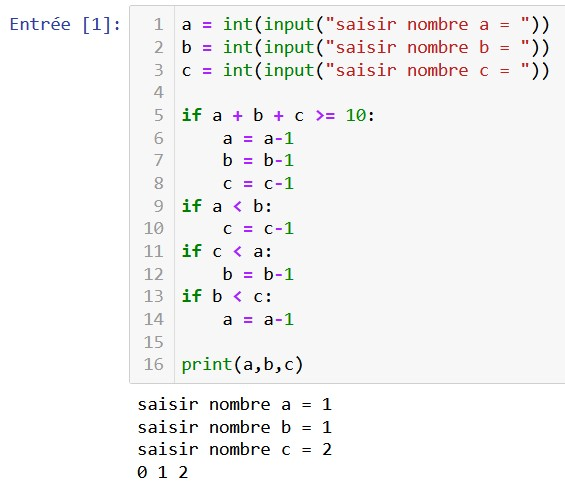
\includegraphics[scale=0.75]{img/activite_1.jpg}
\end{center}

\section*{Partie 1}
\begin{enumerate}
\item Expliquer l'affichage sous le code du programme.
\item On saisit $a=3$, $b=5$ et $c=4$. 

Quelles seront les valeurs affichées des variables $a$, $b$ et $c$ à la fin du programme ?

\end{enumerate}

\section*{Partie 2}

En programmation, on remplace souvent des blocs de code d'un programme par une fonction. En python, une fonction est définie par la syntaxe :

\begin{center}
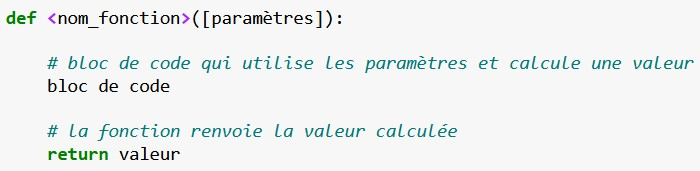
\includegraphics[scale=0.75]{img/activite_2.jpg}
\end{center}

\begin{itemize}[label=\textbullet]
\item le mot clé \textsf{def} informe python que l'on crée une fonction.
\item \textsf{<nom\_fonction>} est le nom de la fonction utilisé pour appeler la fonction.
\item \textsf{([paramètres])} sont les paramètres nécessaires pour calculer une valeur avec la fonction.
\end{itemize}

\begin{enumerate}
\item Il y a dans ce programme des instructions ou des blocs de code qui sont semblables. Lesquels ?

\item La fonction \textsf{calculer(n)} a pour paramètre un nombre \textsf{n} et renvoie la valeur \textsf{n-1}.

\begin{enumerate}
\item Écrire en Python la fonction \textsf{calculer(n)}.
\item Comment et où introduire la fonction \textsf{calculer(n)} dans le programme principal ?
\end{enumerate}

\item La fonction \textsf{saisir(v)} a pour paramètre une chaine de caractères \textsf{v}. Cette fonction provoque la saisie d'un nombre et renvoie ce nombre saisi.

\begin{enumerate}
\item Écrire en Python la fonction \textsf{saisir(v)}.
\item Comment et où introduire la fonction \textsf{saisir(v)} dans le programme principal ?
\end{enumerate}


\item Modifier le programme initial en y ajoutant les deux fonctions \textsf{calculer} et \textsf{saisir}, puis contrôler que l'on retrouve bien les valeurs de la partie 1.

\end{enumerate}

\section*{Approfondir}

Ajouter un test qui vérifie que le nombre saisi par l'utilisateur est bien un nombre. Dans le cas contraire, la valeur du nombre est $0$.

\end{document}
